\documentclass[../../main.tex]{subfiles}


\begin{document}
\subsection*{(a)}
We use the Plugin 'Use Trace Attribute Values' to only select Tickets of type 'Task'. As visualization we then choose 'Explore Event Log'.
This gives us the table below:\\
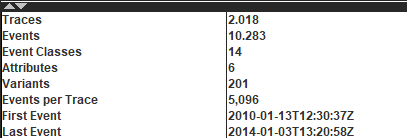
\includegraphics[width=0.5\columnwidth]{img/ProM_a_traces.png}\\
From it we can take that there are 2018 traces, 201 trace variants and 10283 events. We then apply the plugin 'Mine Petri net with Inductive Miner' on this filtered log and make sure we choose 'Inductive Miner - Infrequent (IMf)' as our variant and set it to 20\% by assigning the Noise threshold to 0.20. This results in the following Model:\\
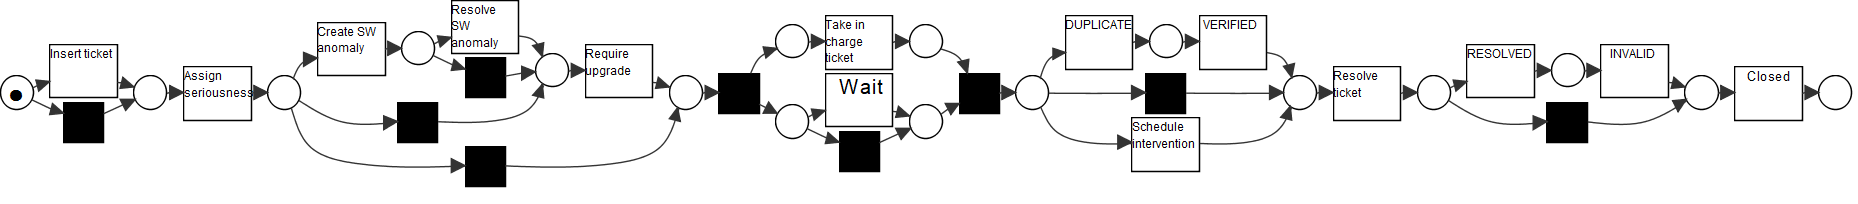
\includegraphics[width=\columnwidth]{img/ProM_a_inductive_miner.png}

\subsection*{(b)}
We use the plugin 'Multi-perspective Process Explorer' on our Petri net from (a). This gives us the following information on fitness and precision:\\
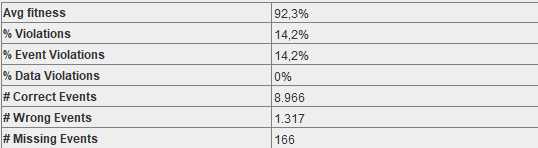
\includegraphics[width=0.5\columnwidth]{img/ProM_b_fitness.png}
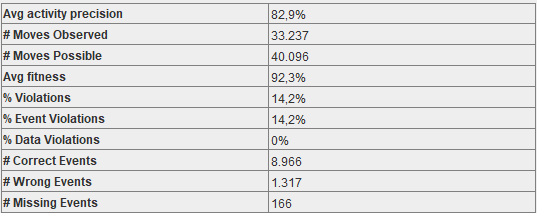
\includegraphics[width=0.5\columnwidth]{img/ProM_b_precision.png}\\
We obtain the percentage of fitting traces by calculating 100\% minus the percentage of violations (100\% - 14.2\%), resulting in 85,8\% fitting traces. Alignment-based fitness (92.3\%) and precision (82.9\%) can be read from the tables above.\\
By using the inductive miner again and adjusting the infrequency parameter to 10\% we obtain a process model with better fitness, precision and more perfectly fitting traces than before. The stats of the new model can be seen below:\\
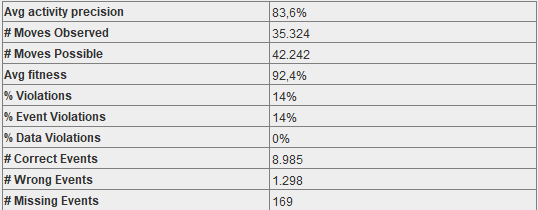
\includegraphics[width=0.5\columnwidth]{img/ProM_b_model_2.png}

\subsection*{(c)}

\end{document}